%%%%%%%%%%%%%%%%%%%%%%%%%%%%%%%%%%%%%%%%%%%%%%%%%%%%%%%%%%%%%%%%%%%%%%%%%
\section{Capa límite}
%%%%%%%%%%%%%%%%%%%%%%%%%%%%%%%%%%%%%%%%%%%%%%%%%%%%%%%%%%%%%%%%%%%%%%%%%

%%%%%%%%%%%%%%%%%%%%%%%%%%%%%%%%%%%%%%%%%%%%%%%%%%%%%%%%%%%%%%%%%%%%%%%%%
\begin{frame}
\frametitle{Capa límite}

Problema 1D isótropo independiente del tiempo
\begin{equation*}
  &  \xi \frac{\partial}{\partial x}\uxi+\mu_t(x)\uxi =   \frac{\mu_s(x)}{2} \int_{-1}^{1}\uxp d\xi' +q(x,\xi)
\end{equation*}
\begin{columns}[t]
\begin{column}{0.4\textwidth}

\scriptsize 
Condiciones de borde de Fresnel
\begin{equation*}
\begin{split}
  &  u(x=0,\xi)=\mathcal{R}(\xi)u(x=0,\xi_R) \; \forall \xi>0\\
  &  u(x=1,\xi)=\mathcal{R}(\xi)u(x=1,\xi_R) \; \forall \xi<0
\end{split}
\end{equation*}

\vspace{0.1\textheight}
$\xi=\cos(\theta)$\\
$\xi \to 0^+$ cuando $\theta \to \pi/2$. 

\end{column}

\begin{column}{0.6\textwidth}
\begin{figure}[h!]
\centering
  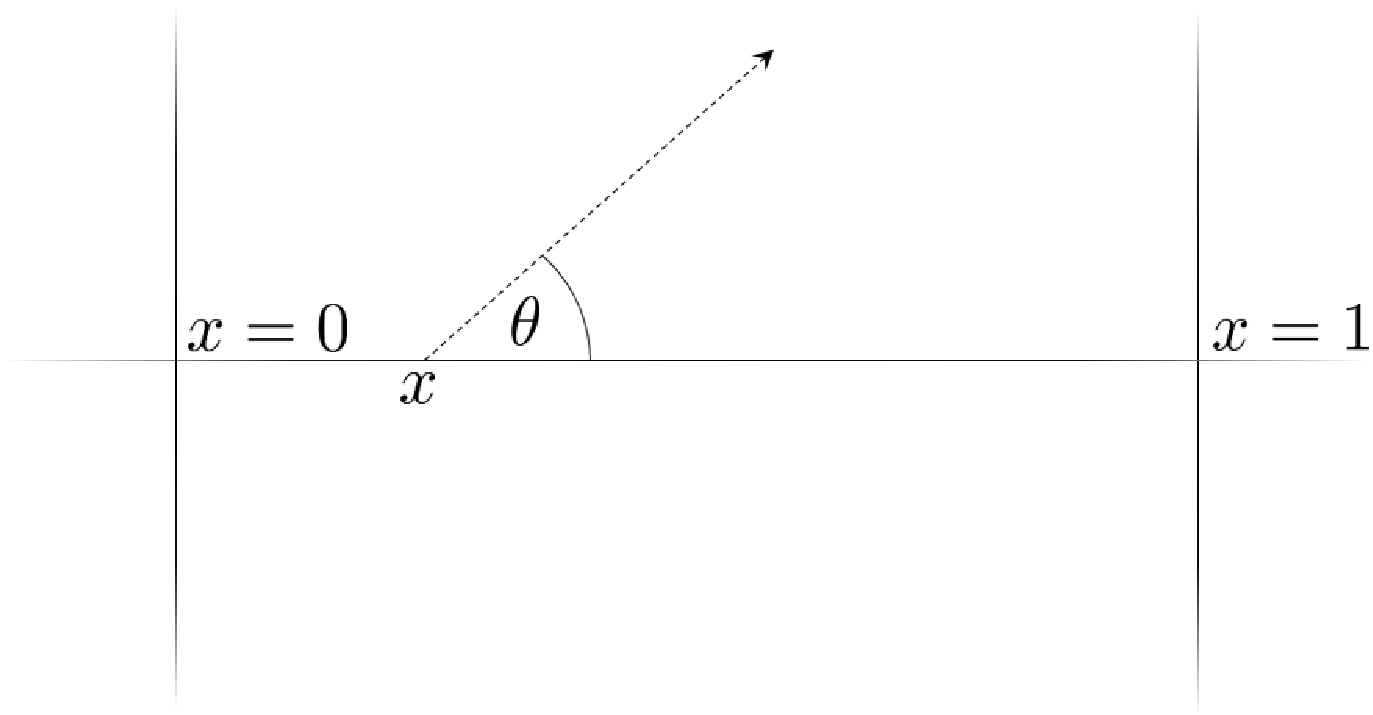
\includegraphics[width=1.0\linewidth]{figuras/geom.pdf}
\end{figure}

\end{column}
\end{columns}

\end{frame}

%%%%%%%%%%%%%%%%%%%%%%%%%%%%%%%%%%%%%%%%%%%%%%%%%%%%%%%%%%%%%%%%%%%%%%%%%
\begin{frame}
\frametitle{Capa límite}

\textit{Solución interna}  $(x,\xi)\to (0^+,0^+)$:

\vspace{0.05\textheight}
Usamos: \\
$X=\frac{x}{\xi},\quad$ $U(X,\xi)=u(\xi X,\xi),\quad$ 
$U(X,\xi) \sim U_0(X,\xi)$

%\vspace{0.05\textheight}
\begin{equation*}
\begin{split}
 \frac{\partial U_0(X,\xi)}{\partial X} + \mu_t(0) U_0(X,\xi)=\frac{\mu_s(0)}{2} 
\int_{-1}^{1} U_0\left(\frac{\xi X}{\xi'},\xi'\right) d\xi' +q(0,\xi),
\end{split}
\end{equation*}

\begin{equation*}
  u(x,\xi)\sim u_0(x,\xi) = U_0(x/\xi,\xi)
\end{equation*}

\end{frame}
%%%%%%%%%%%%%%%%%%%%%%%%%%%%%%%%%%%%%%%%%%%%%%%%%%%%%%%%%%%%%%%%%%%%%%%%%
\begin{frame}
\frametitle{Capa límite}

Utilizando el factor integrante, y definiendo
\begin{equation*}
I(x,\xi) = \int_0^{x} e^{\frac{ \mu_t(0) y}{\xi}}\left[\frac{\mu_s(0)}{2} \int_{-1}^1u_0(y,\xi')d\xi'+q(0,\xi)\right]dy,
\end{equation*}
se obtiene
\begin{equation*}
 u_0(x,\xi) = \frac{\textcolor{red}{e^{-\mu_t(0)x/\xi}}}{\xi} \Big[\xi u(0,\xi)+I(x,\xi)\Big] .
\end{equation*}

\end{frame}

%%%%%%%%%%%%%%%%%%%%%%%%%%%%%%%%%%%%%%%%%%%%%%%%%%%%%%%%%%%%%%%%%%%%%%%%%
\begin{frame}
\frametitle{Capa límite}
Estructura de capa límite con $\mu_s(x)=0$.
\begin{columns}[c]
\begin{column}{0.5\textwidth}
$u(x,\xi)=$
\begin{equation*}
\begin{split}
\begin{cases}
\displaystyle \frac{q}{\mu_a}\left[1-\frac{\eta(\xi)}{ e^{\mu_a x / \xi}}\right]&\forall\xi>0,\\[8pt]
\displaystyle  \frac{q}{\mu_a}\left[1- \frac{\eta(\xi)}{e^{\mu_a (x-1) / \xi}} \right]&\forall\xi<0,
\end{cases}
\end{split}
\end{equation*}

\begin{equation*}
\eta(\xi)=\frac{\mathcal{R}(|\xi|)-1}{\mathcal{R}(|\xi|)e^{-\mu_a/|\xi|}-1}
\end{equation*}

\end{column}
\begin{column}{0.5\textwidth}
\begin{figure}[h!]
\centering
  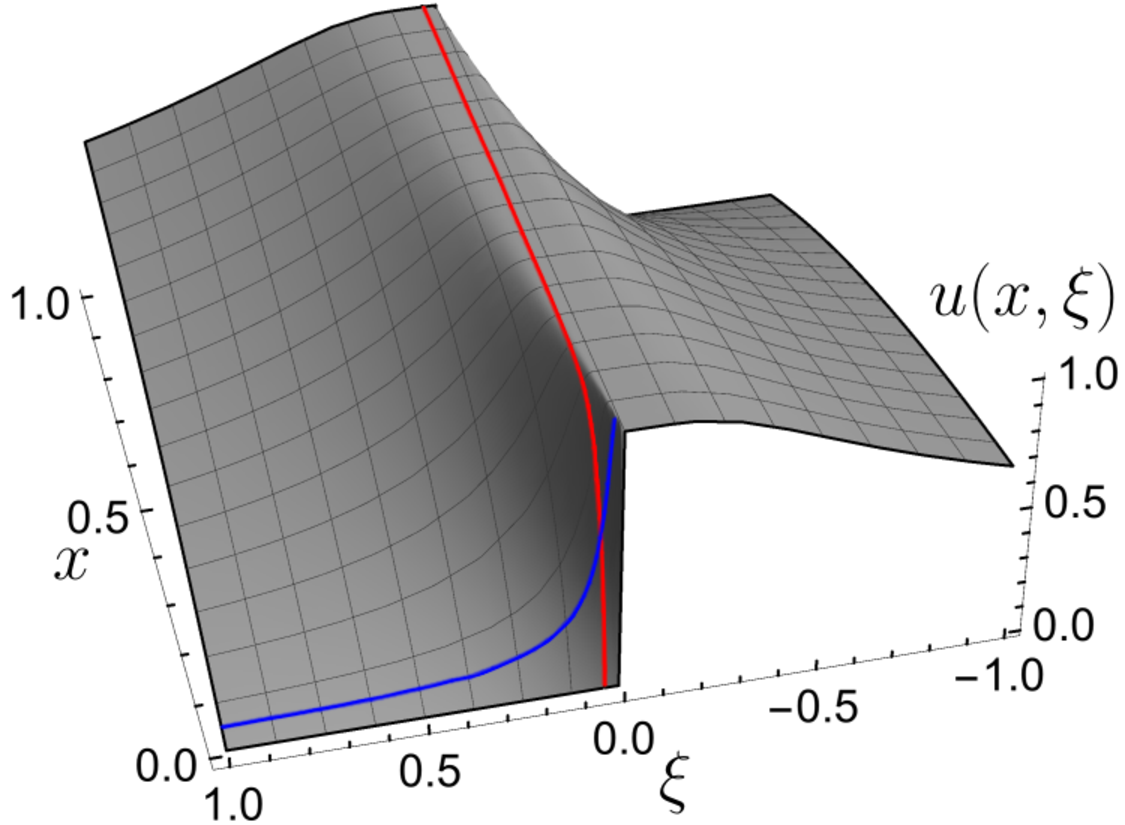
\includegraphics[width=1.1\linewidth]{figuras/Analytic_lay_3.pdf}
 \label{fig:ansol}
\end{figure}
\centering
 $\mathcal{R}(\xi)=0$
\end{column}
\end{columns}
\end{frame}


%%%%%%%%%%%%%%%%%%%%%%%%%%%%%%%%%%%%%%%%%%%%%%%%%%%%%%%%%%%%%%%%%%%%%%%%%

\begin{frame}
\frametitle{Capa límite: cambio de variable}

\begin{itemize}

\item Error de cuadratura de $\ell$-puntos 
decrece como $32V/15\pi j (2\ell+1-j)^j$ siempre que la derivada 
$j$-ésima esté acotada por la constante $V$. 

\item Proponemos el cambio de variable  $\xi'=r^p$.

\item Buscamos una cota $V$ 
para la derivada
\begin{equation*}
\begin{split}
\left | \frac{\partial^j }{\partial r^j}\left[ u(x,r^p) r^{p-1}\right]
\right|\leq W r^{p-j-1}
\end{split}
\end{equation*}
para alguna constante $W$. 

\item Llamando $V = W r^{p-j-1}$  
se obtiene la cota deseada, {\em uniforme 
para todo $x$ y $r$ }.

\end{itemize}


\end{frame}


%%%%%%%%%%%%%%%%%%%%%%%%%%%%%%%%%%%%%%%%%%%%%%%%%%%%%%%%%%%%%%%%%%%%%%%%%

\begin{frame}
\frametitle{Capa límite: cambio de variable}

\begin{center}
  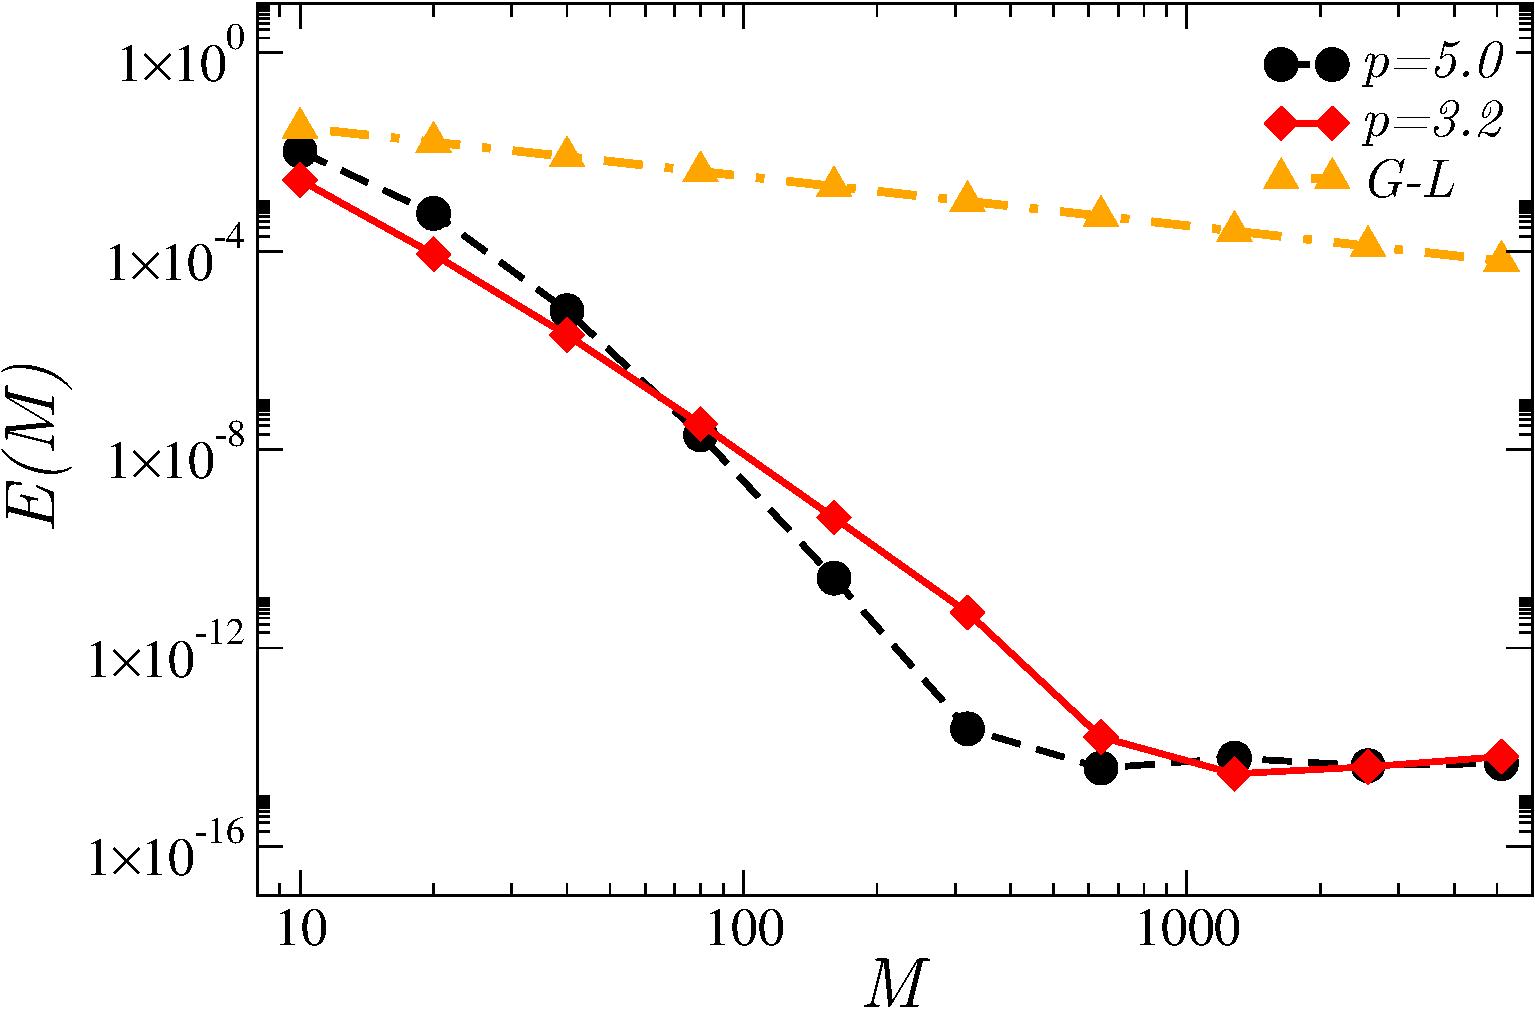
\includegraphics[width=0.8\textwidth]{figuras/quads.pdf}\\

$E(M)=\text{max}_x |\sum_{i=1}^M w_i u(x,\xi_i)-I^{\text{an}}(x)|$ con $\mathcal{R}(\xi)=0$.
 \end{center}


\end{frame}

%%%%%%%%%%%%%%%%%%%%%%%%%%%%%%%%%%%%%%%%%%%%%%%%%%%%%%%%%%%%%%%%%%%%%%%%%

\begin{frame}
\frametitle{Capa límite: cambio de variable espacial}
\begin{columns}[c]

\begin{column}{0.55\textwidth}
$v=\log(\frac{x}{1-x})$

\begin{figure}
  \includegraphics[width=1.0\textwidth]{figuras/puntos.eps}
\end{figure}

\end{column}

\begin{column}{0.45\textwidth}
\scriptsize
\begin{equation*}
\begin{split}
&\frac{\partial}{\partial t}\uvi+\xi(2+2\cosh(v)) \frac{\partial}{\partial v}\uvi\\
&+\st\uvi=\sct \int_{-1}^{1} \uvp d\xi'+q, \\
\end{split}
\end{equation*}

\vspace{0.025\textheight}
\begin{equation*}
\begin{split}
&u(v,\xi,t_{\text{min}})=0,\\
&u(v_{\text{min}},\xi,t)=u_{0}(x'_{\text{min}},\xi,t) \; \forall \xi>0,\\
&u(v_{\text{max}},\xi,t)=u_{0}(x'_{\text{max}},\xi,t) \; \forall \xi<0.
\end{split}
\end{equation*}
\end{column}
\end{columns}

\end{frame}


%%%%%%%%%%%%%%%%%%%%%%%%%%%%%%%%%%%%%%%%%%%%%%%%%%%%%%%%%%%%%%%%%%%%%%%%%

\begin{frame}
\frametitle{Capa límite: convergencia}

\begin{columns}
\begin{column}{0.33\textwidth}
  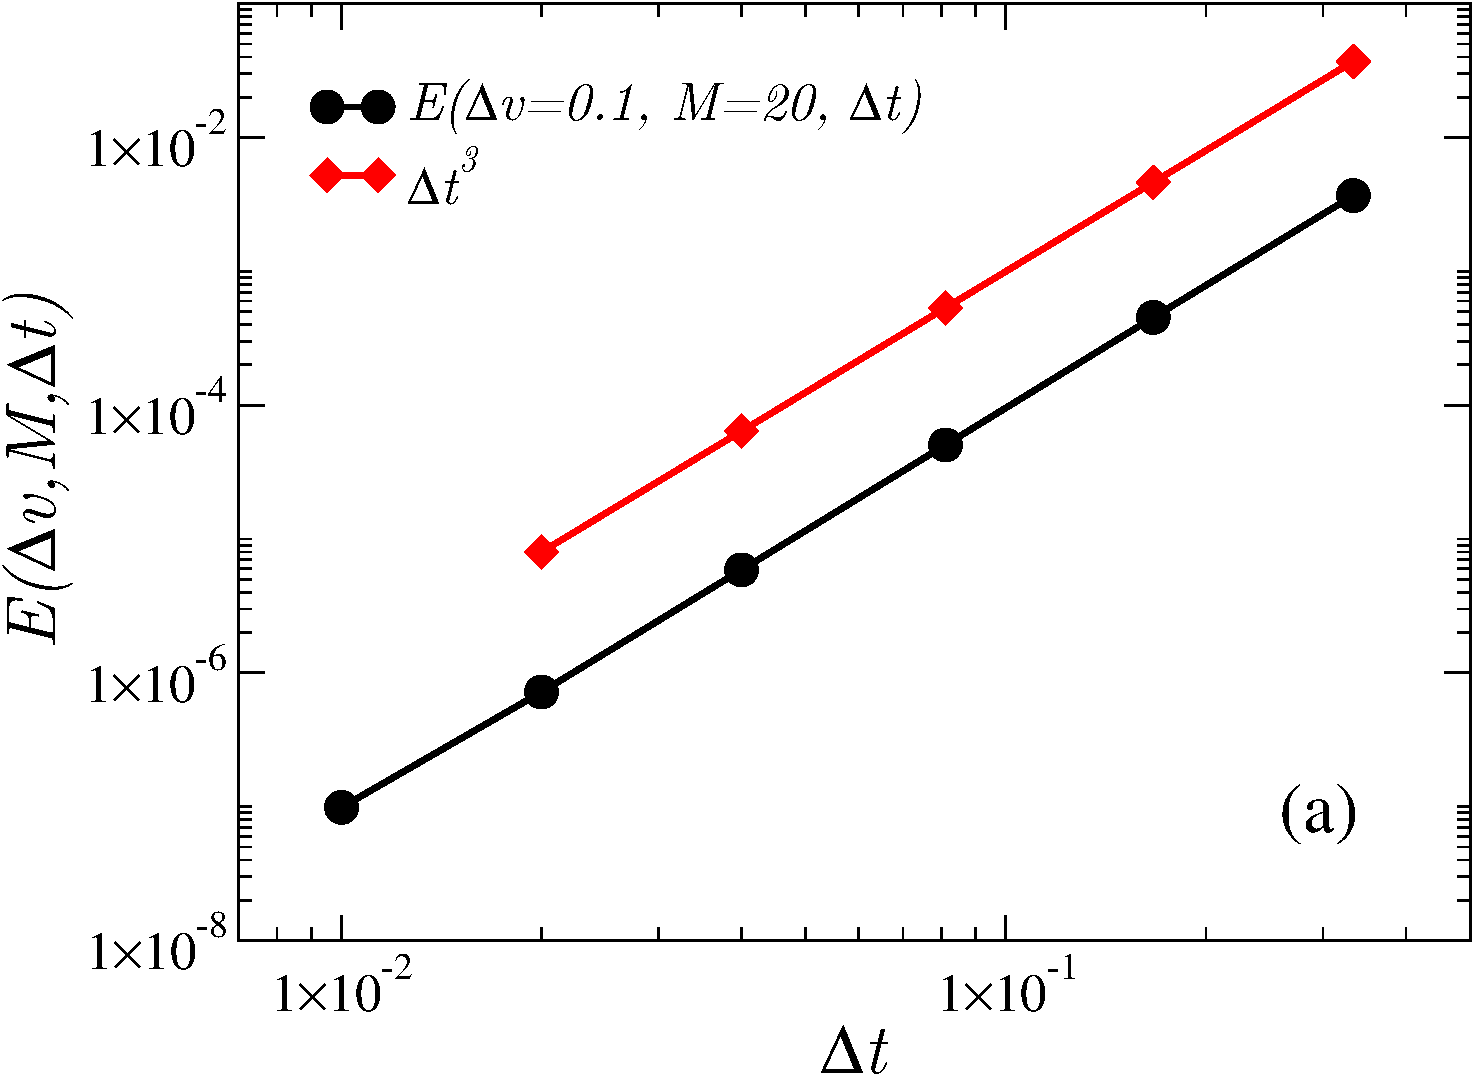
\includegraphics[width=1.1\textwidth]{figuras/errdt.pdf}
\end{column}
\begin{column}{0.33\textwidth}
  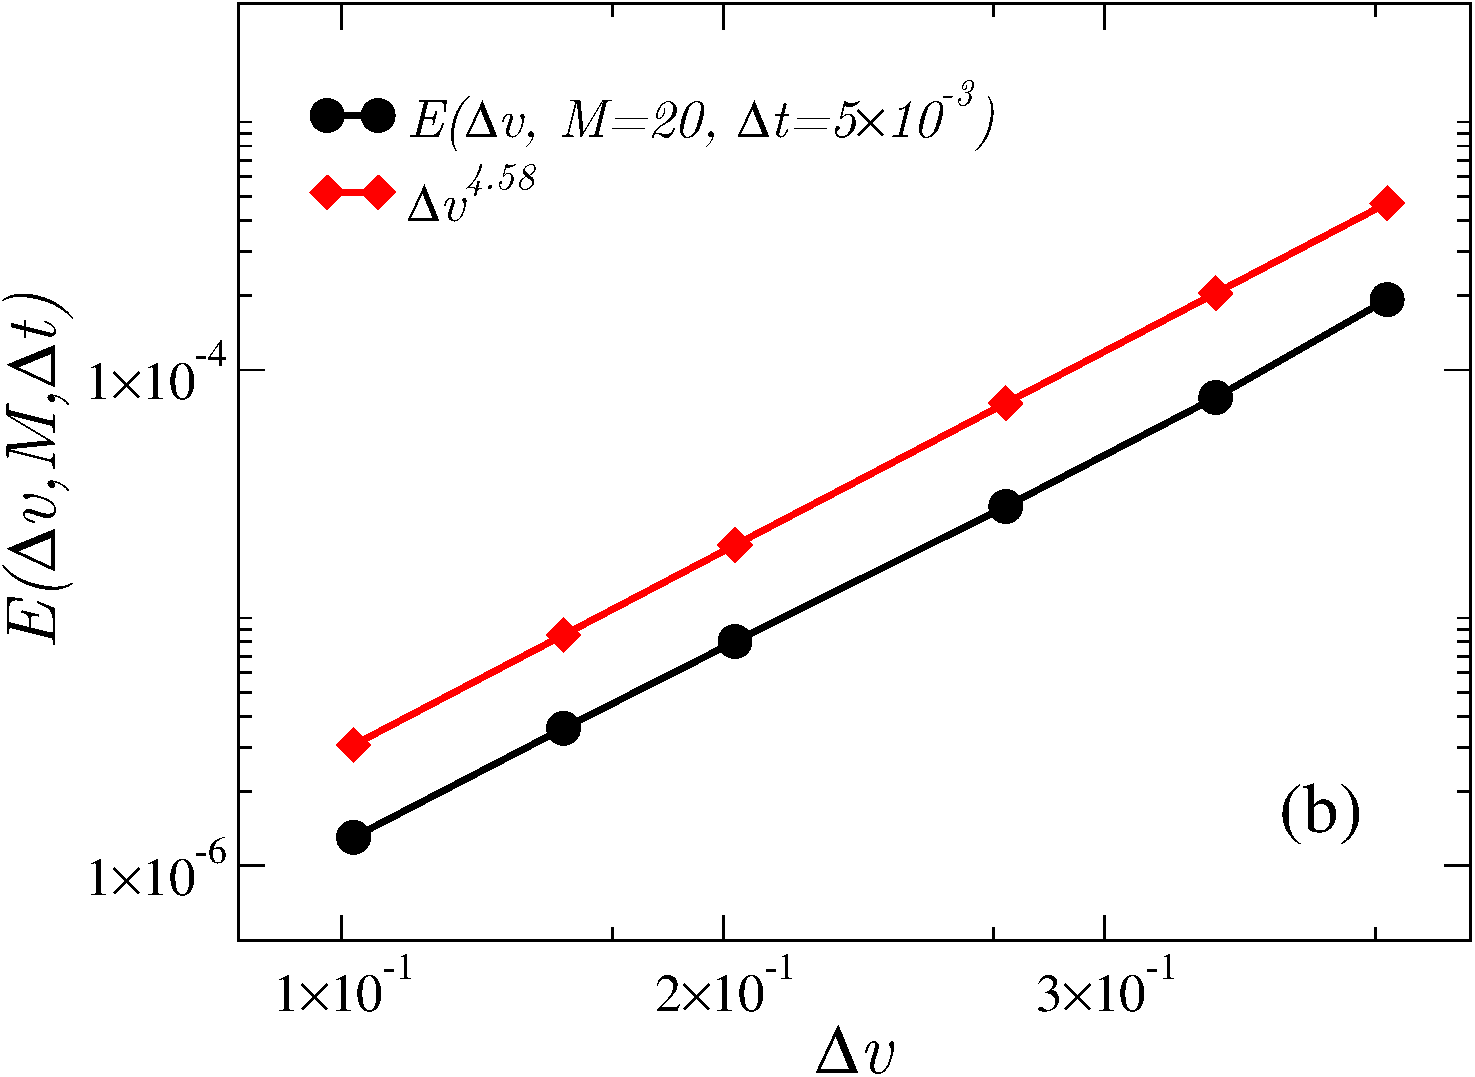
\includegraphics[width=1.1\textwidth]{figuras/errdx.pdf}
\end{column}
\begin{column}{0.33\textwidth}
  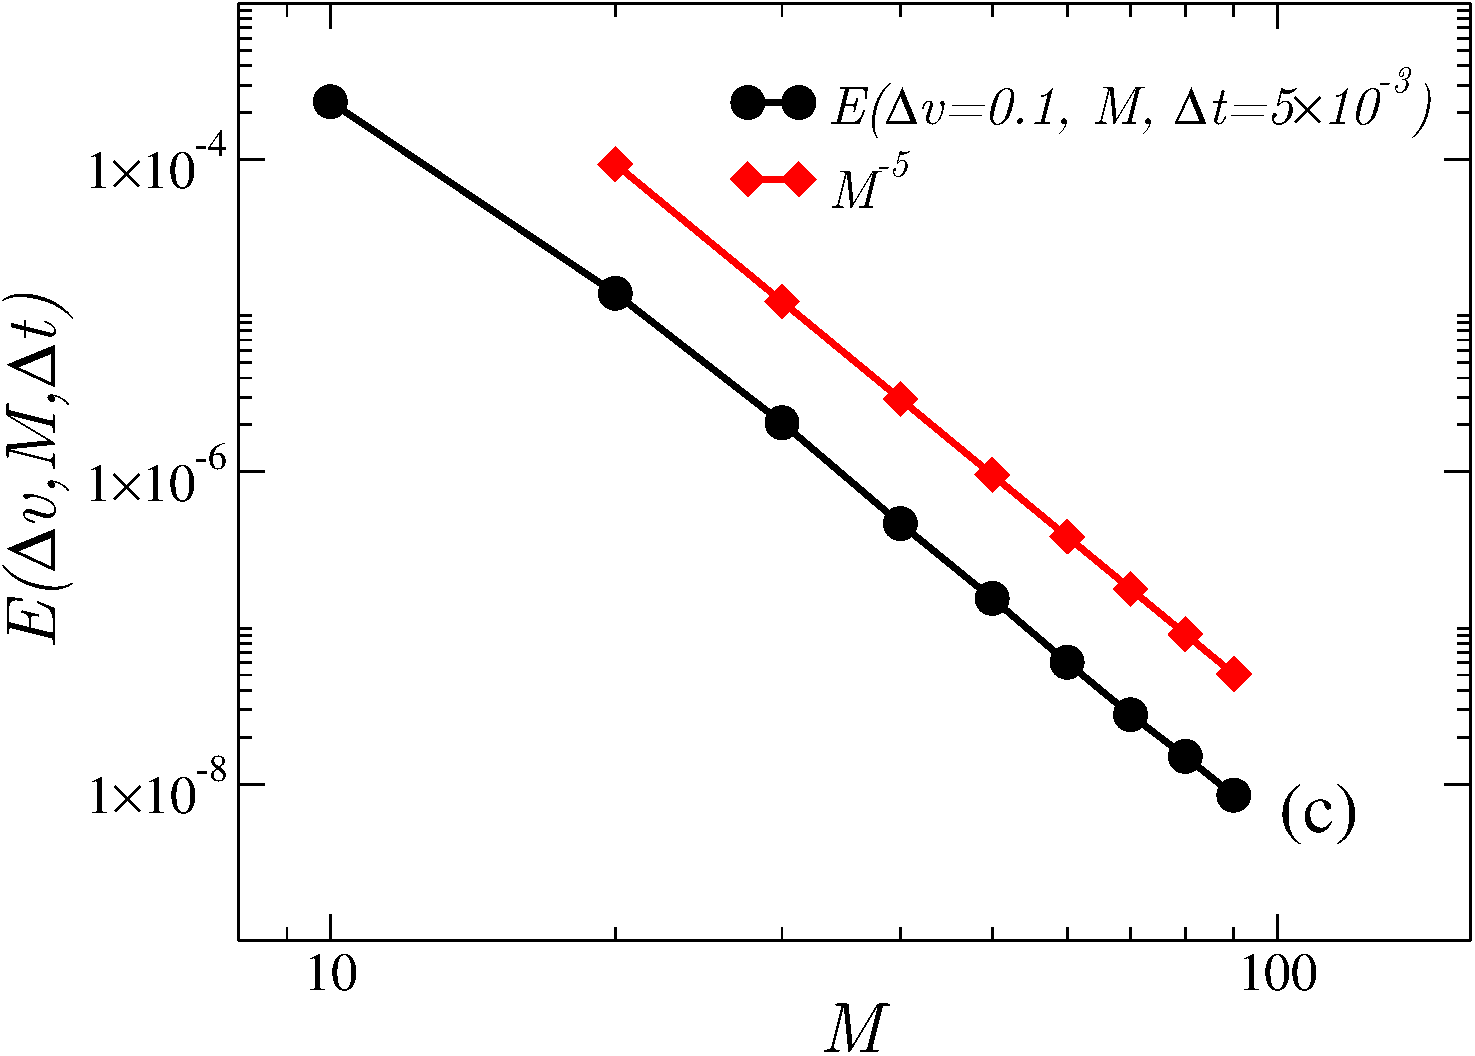
\includegraphics[width=1.1\textwidth]{figuras/xiconv.pdf}
\end{column}
\end{columns}

\end{frame}

%%%%%%%%%%%%%%%%%%%%%%%%%%%%%%%%%%%%%%%%%%%%%%%%%%%%%%%%%%%%%%%%%%%%%%%%%

%\begin{frame}
%\frametitle{Capa límite}
%\begin{columns}[t]
%\begin{column}{0.33\textwidth}
%\centering
%  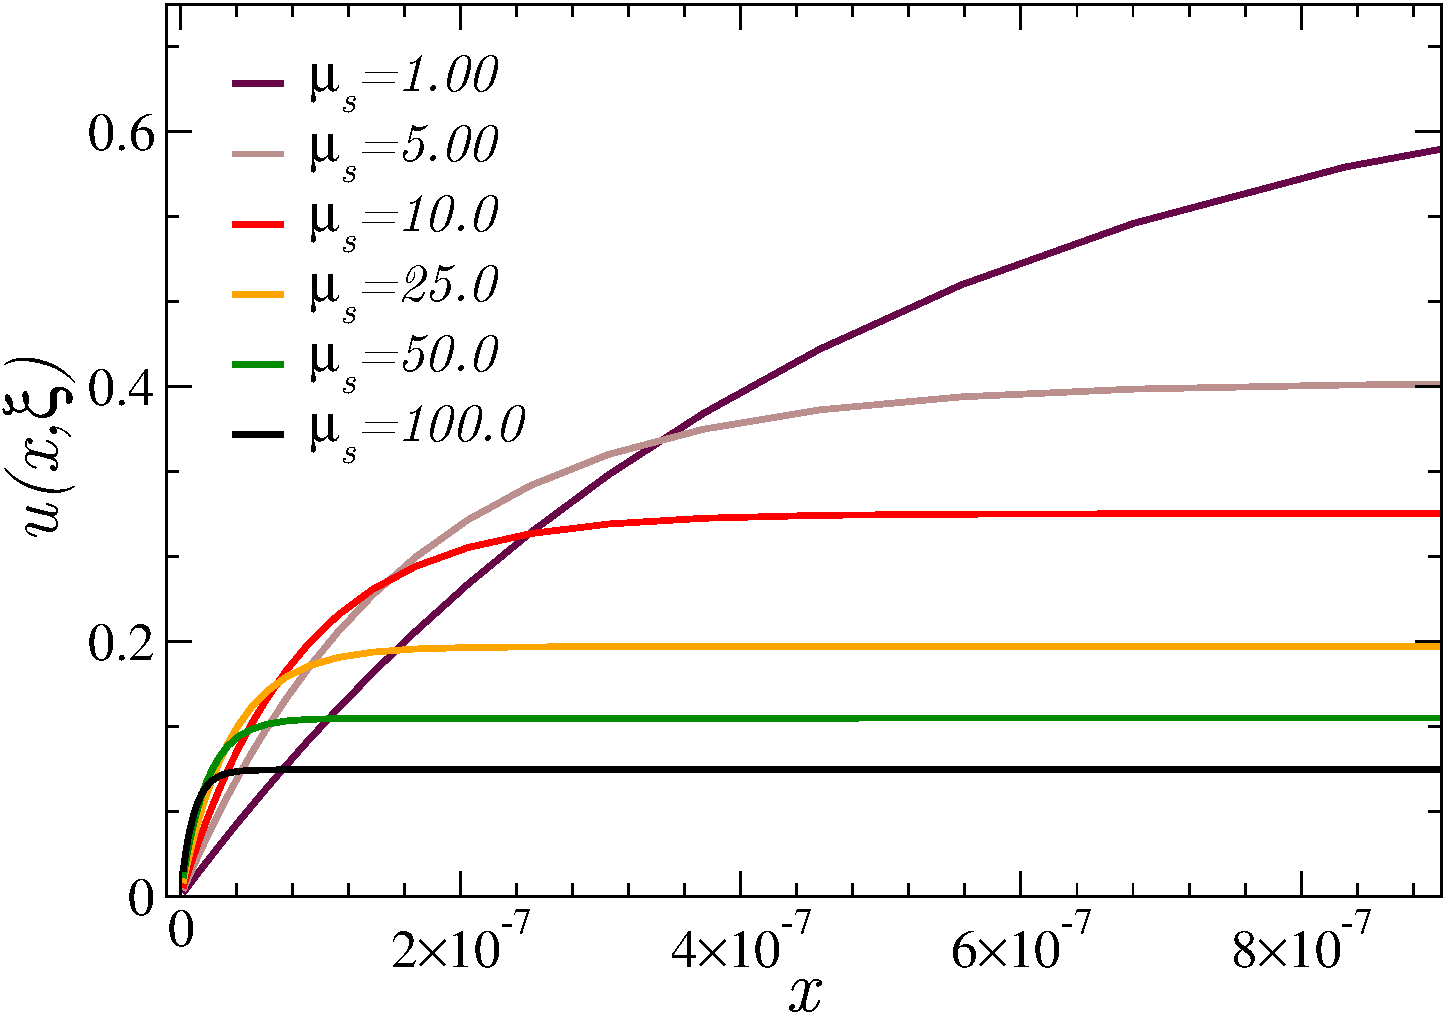
\includegraphics[width=1.1\textwidth]{figuras/blayers.pdf}\\
%   $\mu_a=q=1$
%\end{column}
%\begin{column}{0.33\textwidth}
%\centering
%  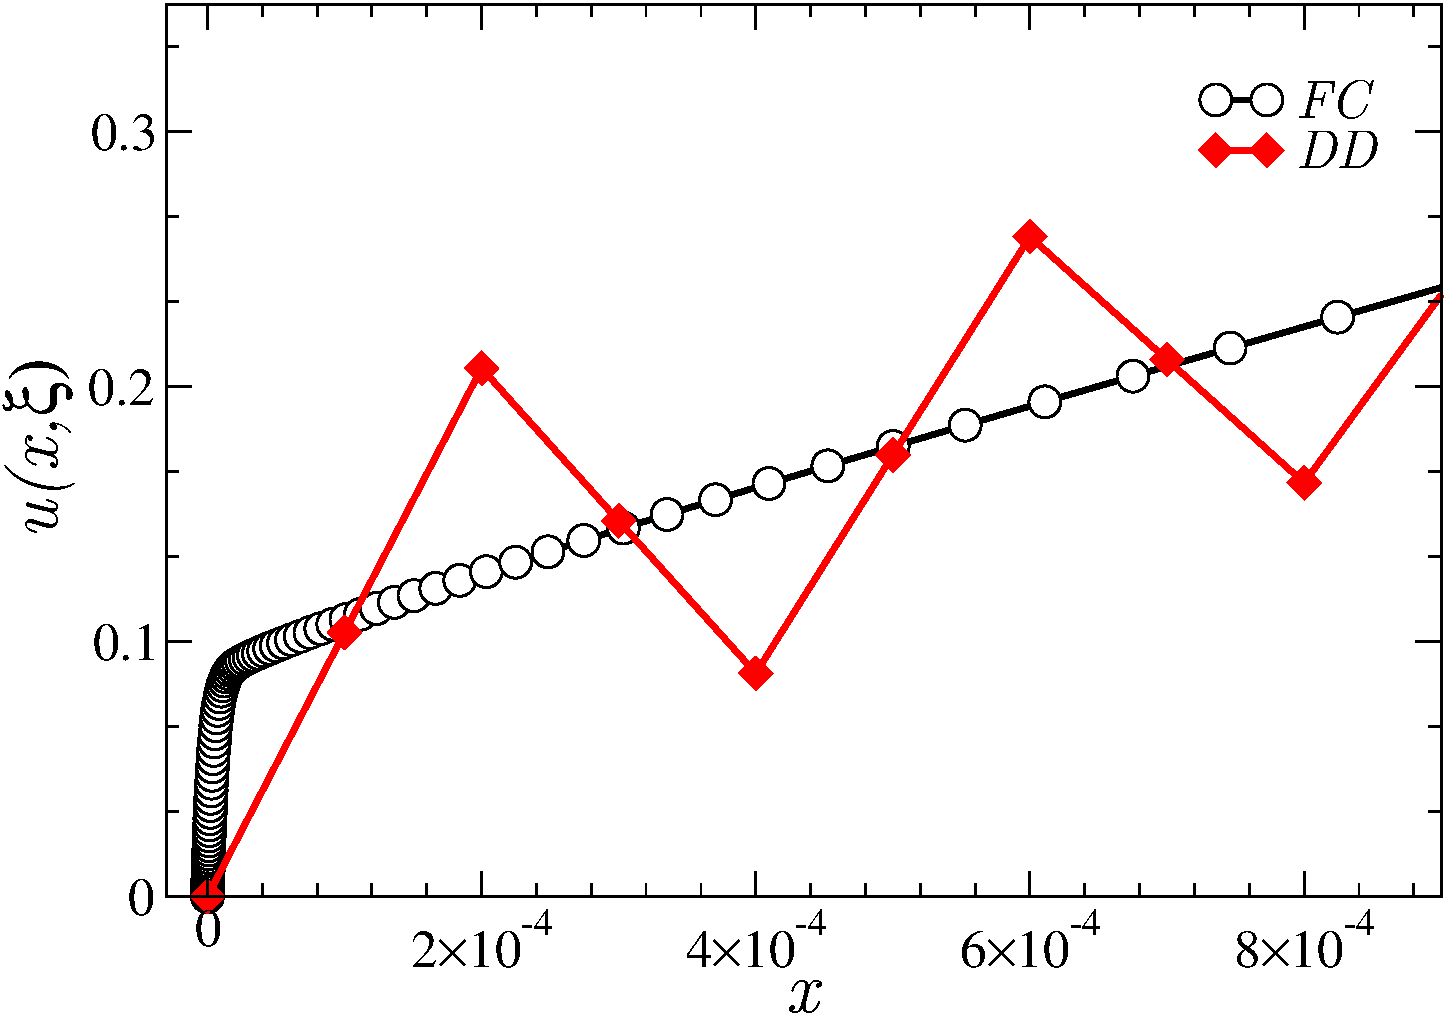
\includegraphics[width=1.1\textwidth]{figuras/layerlar.pdf}\\
%  FC: $N=400$,\\ DD: $N=10000$.
%\end{column}
%\begin{column}{0.33\textwidth}
%\centering
%  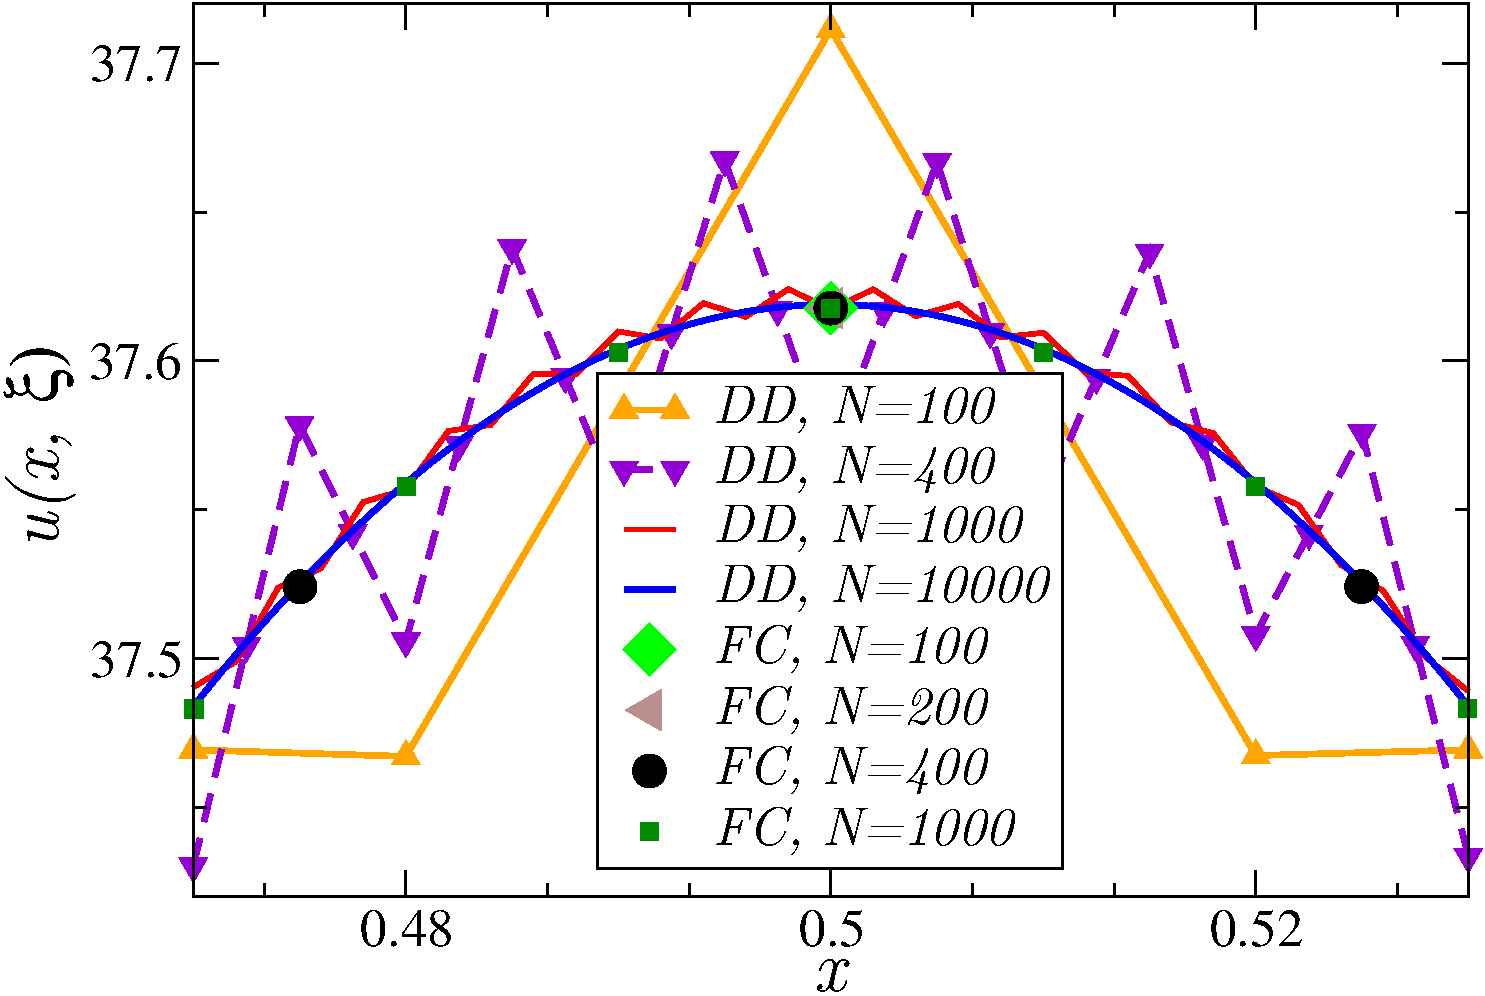
\includegraphics[width=1.15\textwidth]{figuras/conv_2-eps-converted-to.pdf}\\
%  Lejos de la región de capa límite.
%\end{column}
%\end{columns}


%\end{frame}

%%%%%%%%%%%%%%%%%%%%%%%%%%%%%%%%%%%%%%%%%%%%%%%%%%%%%%%%%%%%%%%%%%%%%%%%%

\begin{frame}
\frametitle{Capa límite}
%\begin{columns}[t]
%\begin{column}{0.5\textwidth}
\centering
  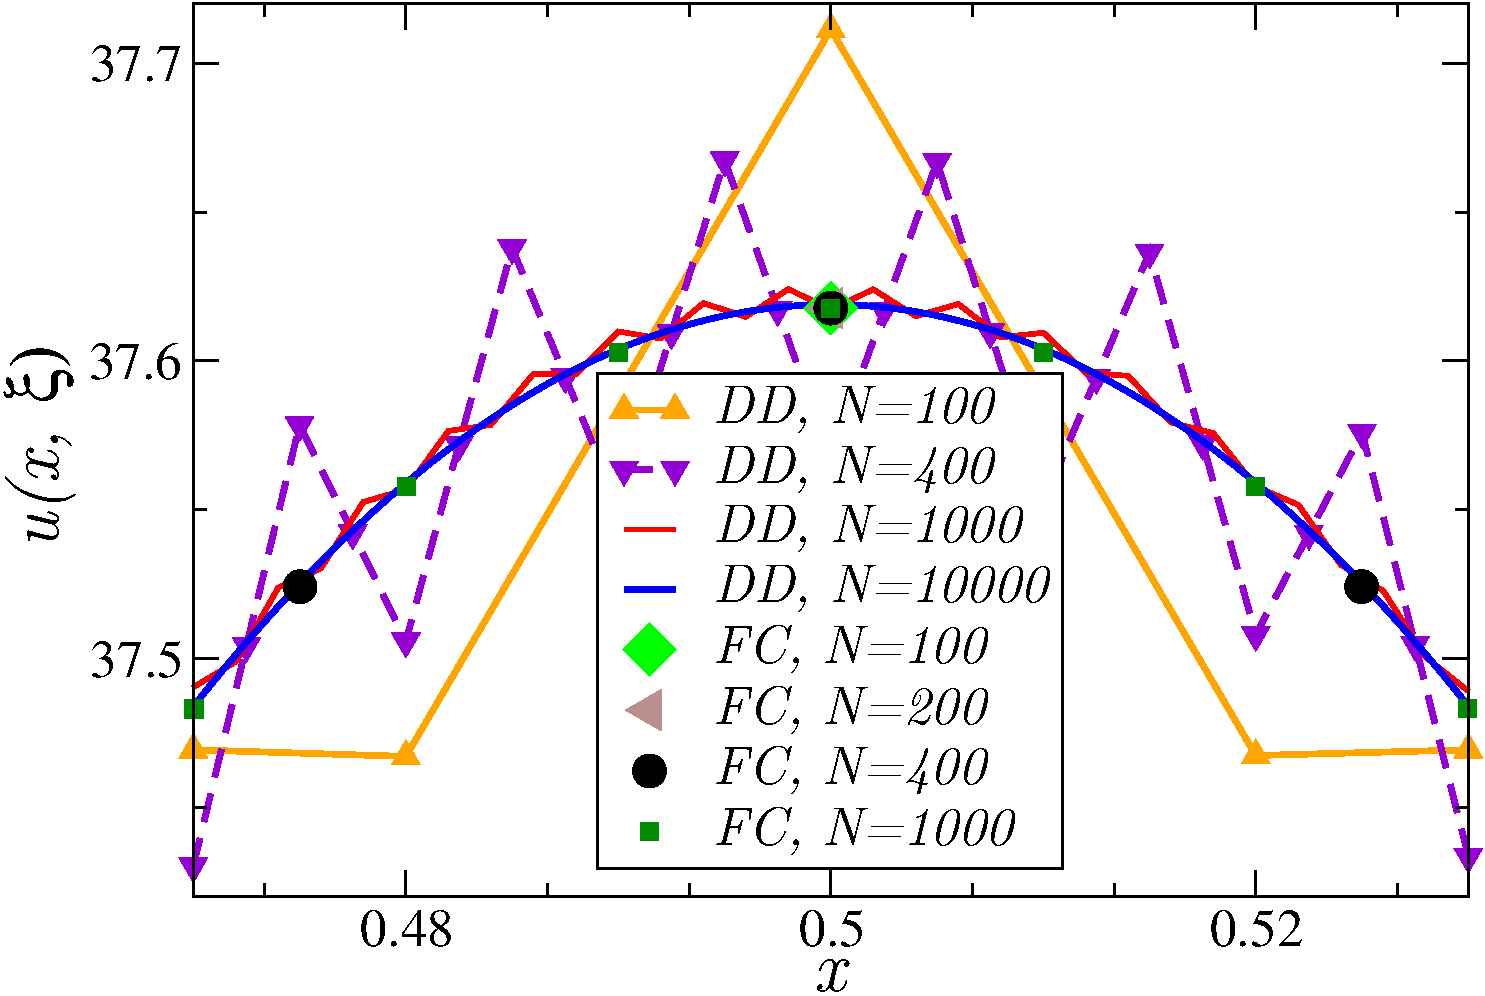
\includegraphics[width=1.0\textwidth]{figuras/conv_2-eps-converted-to.pdf}\\
%\end{column}
%\begin{column}{0.5\textwidth}
%\centering
%  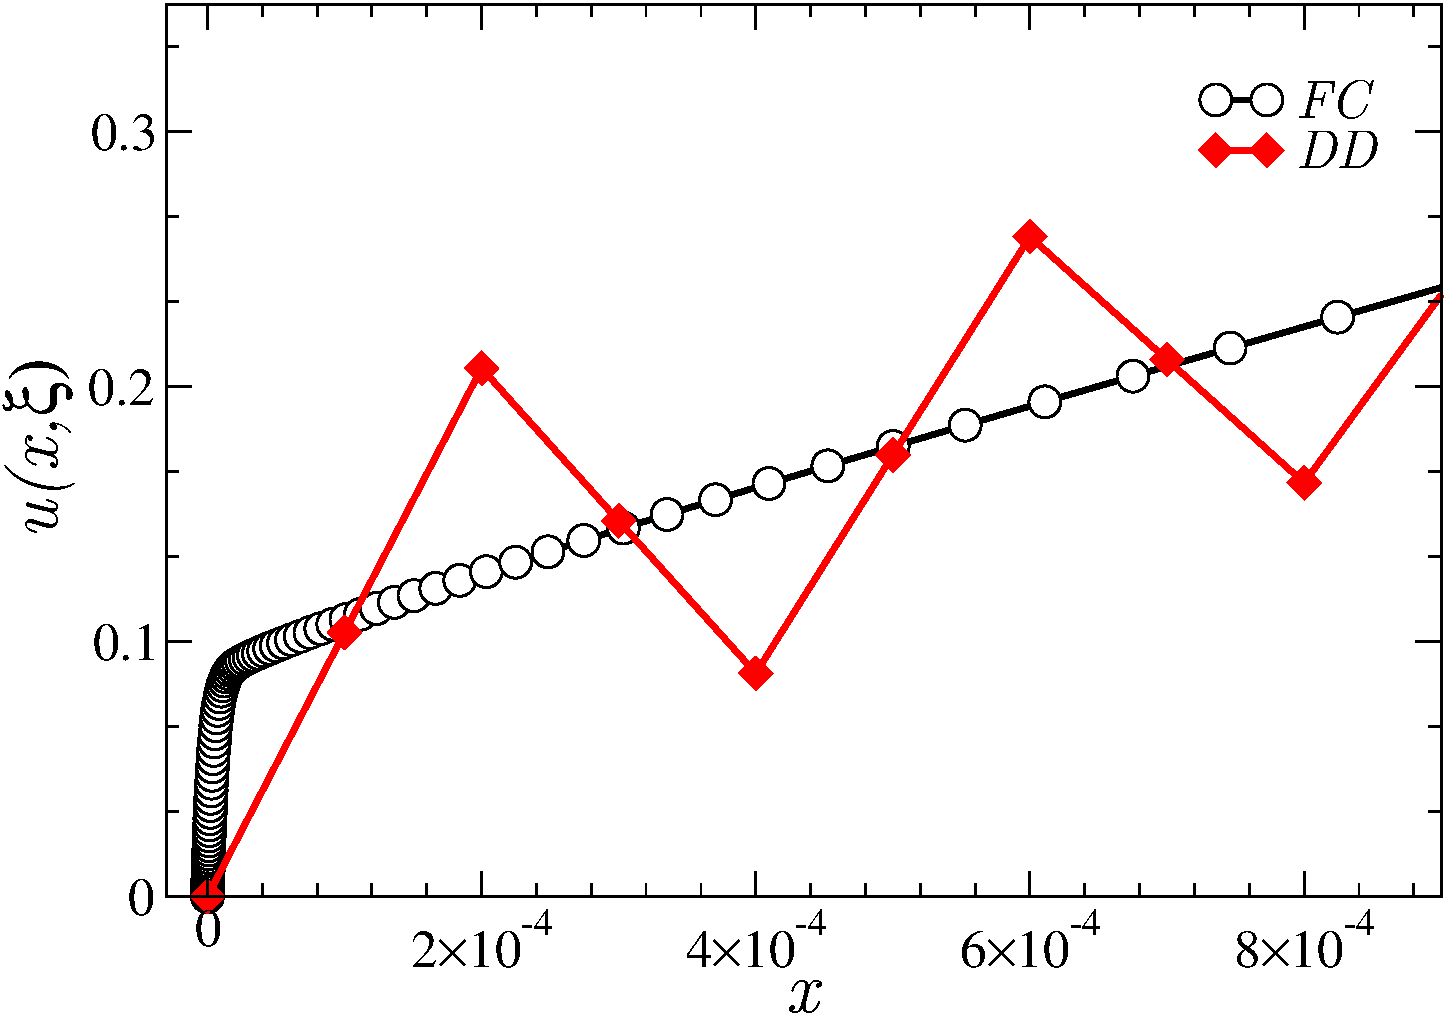
\includegraphics[width=1.0\textwidth]{figuras/layerlar.pdf}\\
%  FC: $N=400$, DD: $N=10000$.
%\end{column}
%\end{columns}


\end{frame}


%%%%%%%%%%%%%%%%%%%%%%%%%%%%%%%%%%%%%%%%%%%%%%%%%%%%%%%%%%%%%%%%%%%%%%%%%

\begin{frame}
\frametitle{Capa límite}
%\begin{columns}[t]
%\begin{column}{0.5\textwidth}
\centering
  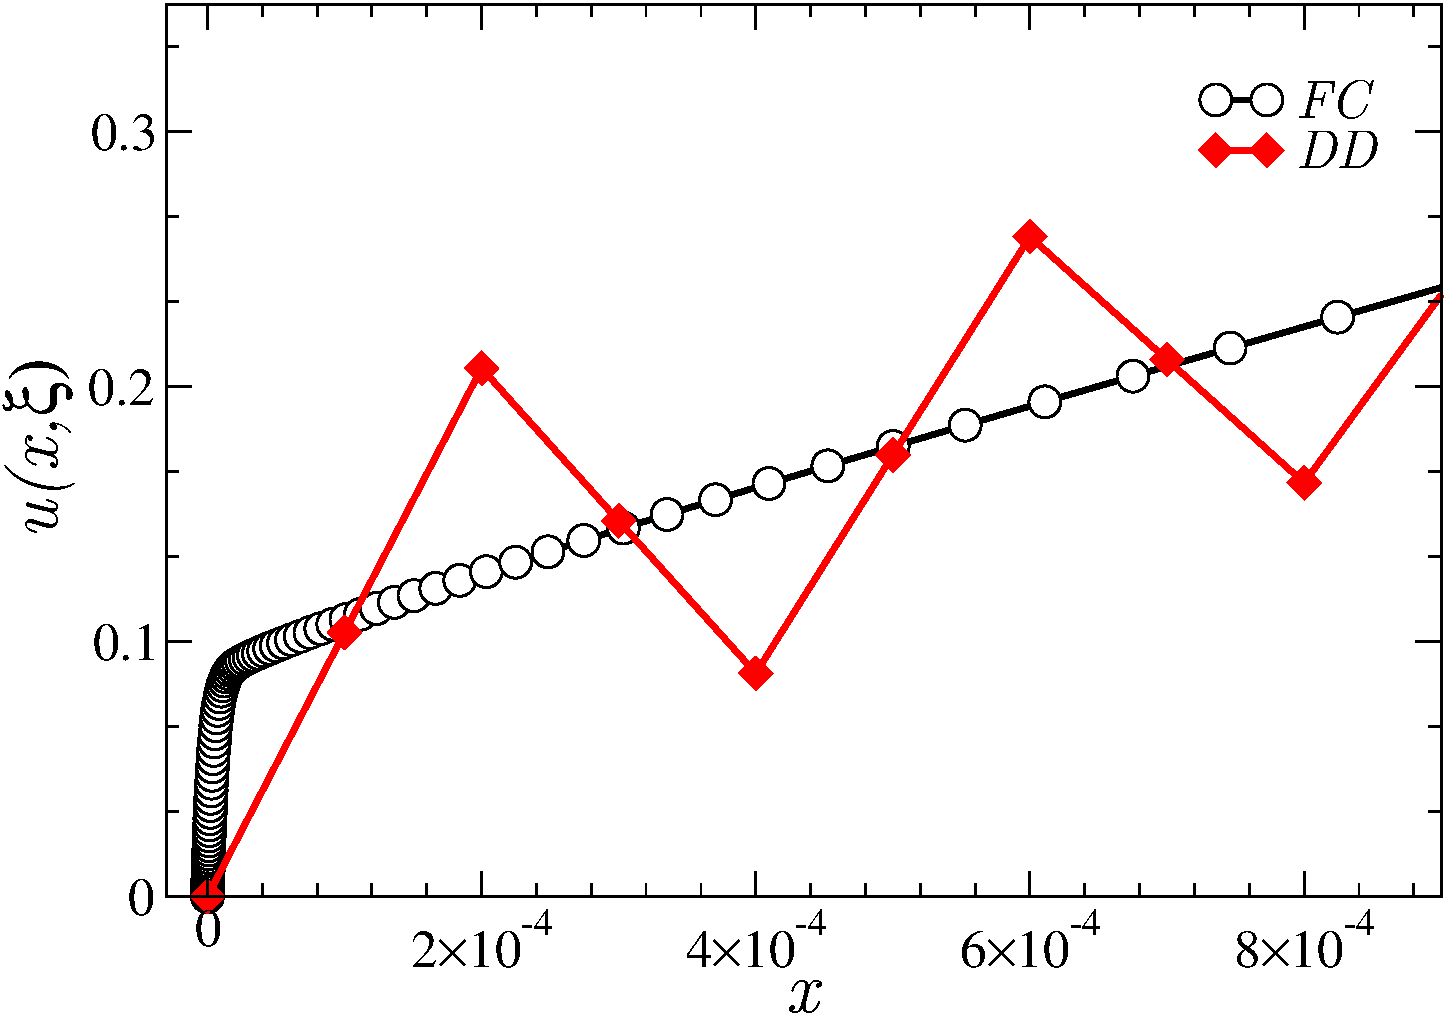
\includegraphics[width=1.0\textwidth]{figuras/layerlar.pdf}\\
FC: $N=400$, DD: $N=10000$.
%\end{column}
%\begin{column}{0.5\textwidth}
%\centering
%  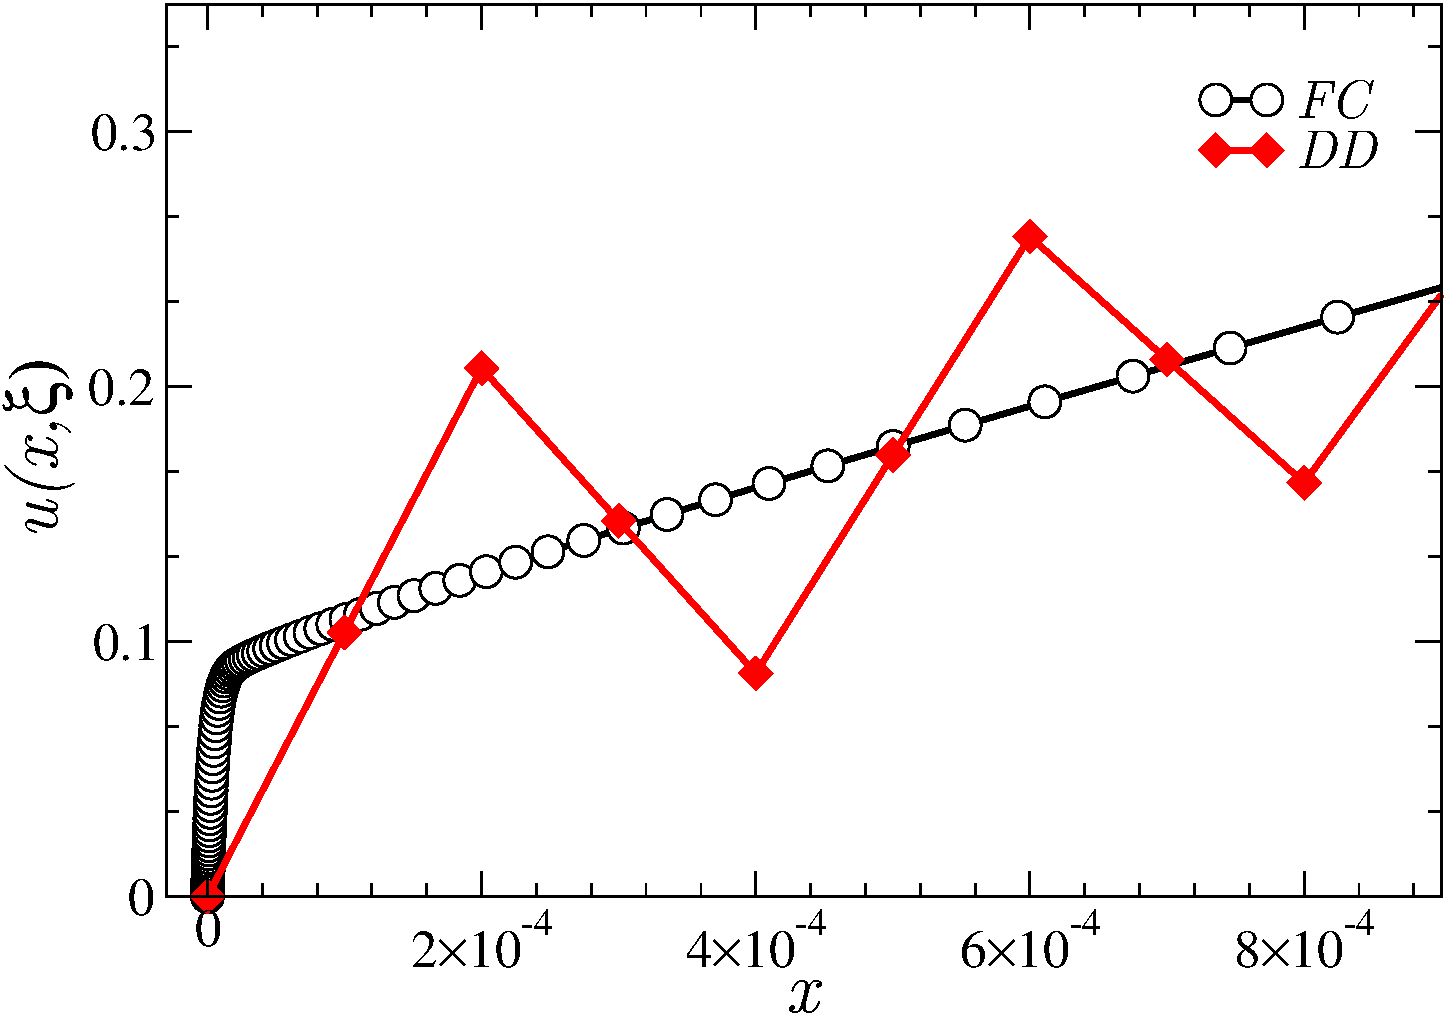
\includegraphics[width=1.0\textwidth]{figuras/layerlar.pdf}\\
%  FC: $N=400$, DD: $N=10000$.
%\end{column}
%\end{columns}


\end{frame}

%%%%%%%%%%%%%%%%%%%%%%%%%%%%%%%%%%%%%%%%%%%%%%%%%%%%%%%%%%%%%%%%%%%%%%%%%



\begin{frame}
\frametitle{Capa límite}
%\begin{columns}[t]
%\begin{column}{0.33\textwidth}
%\centering
%  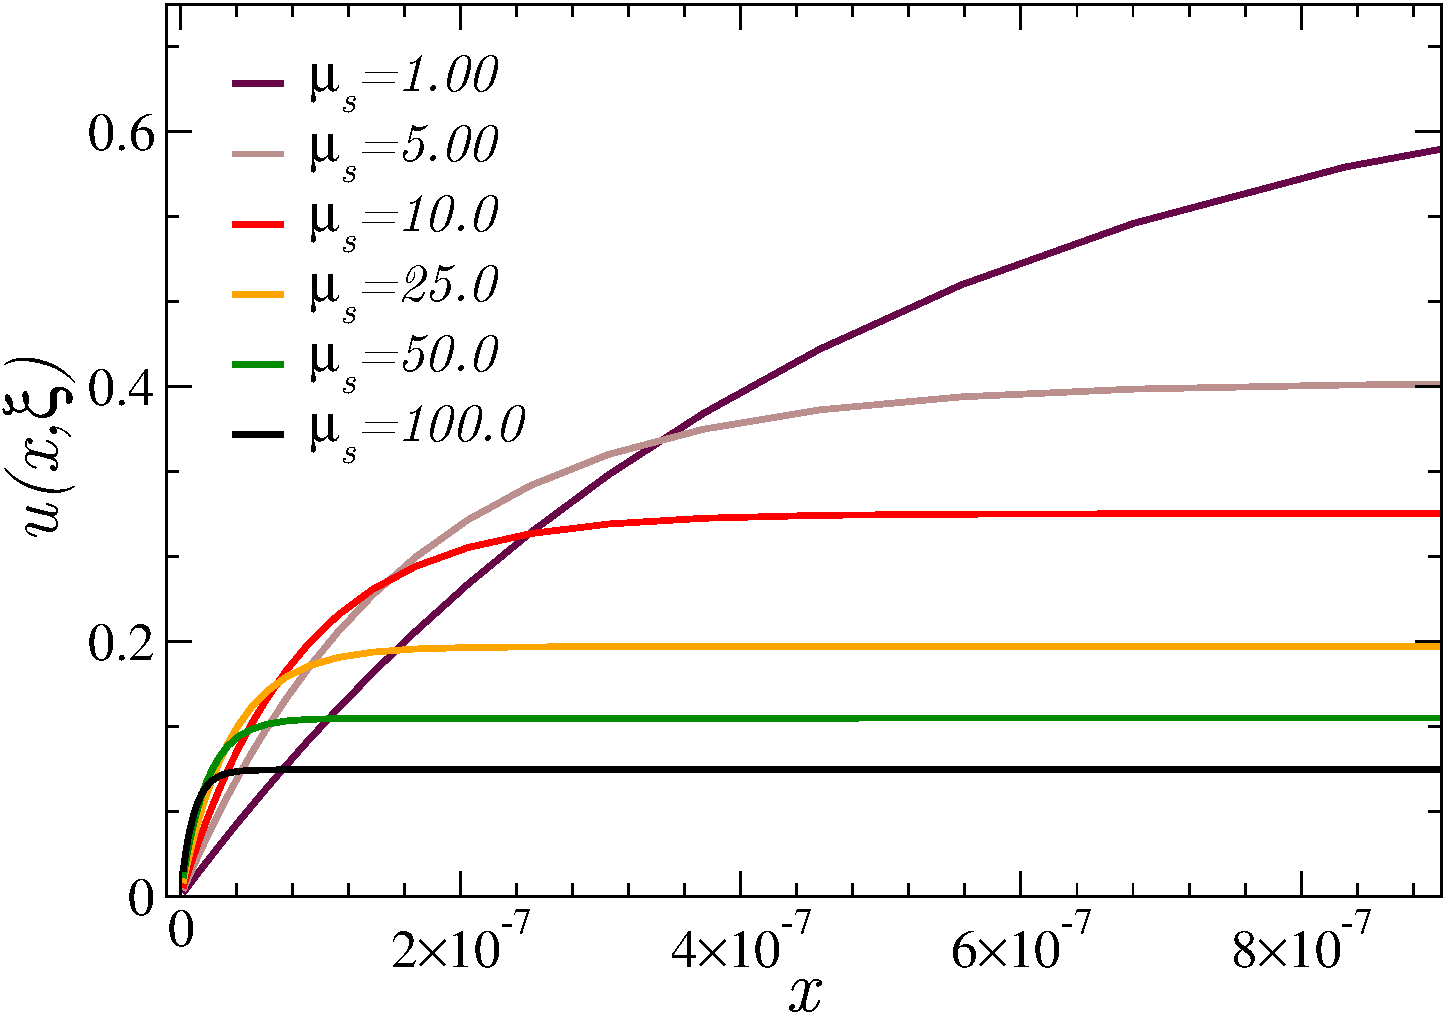
\includegraphics[width=1.1\textwidth]{figuras/blayers.pdf}\\
%   $\mu_a=q=1$
%\end{column}
%\begin{column}{0.5\textwidth}
\centering
  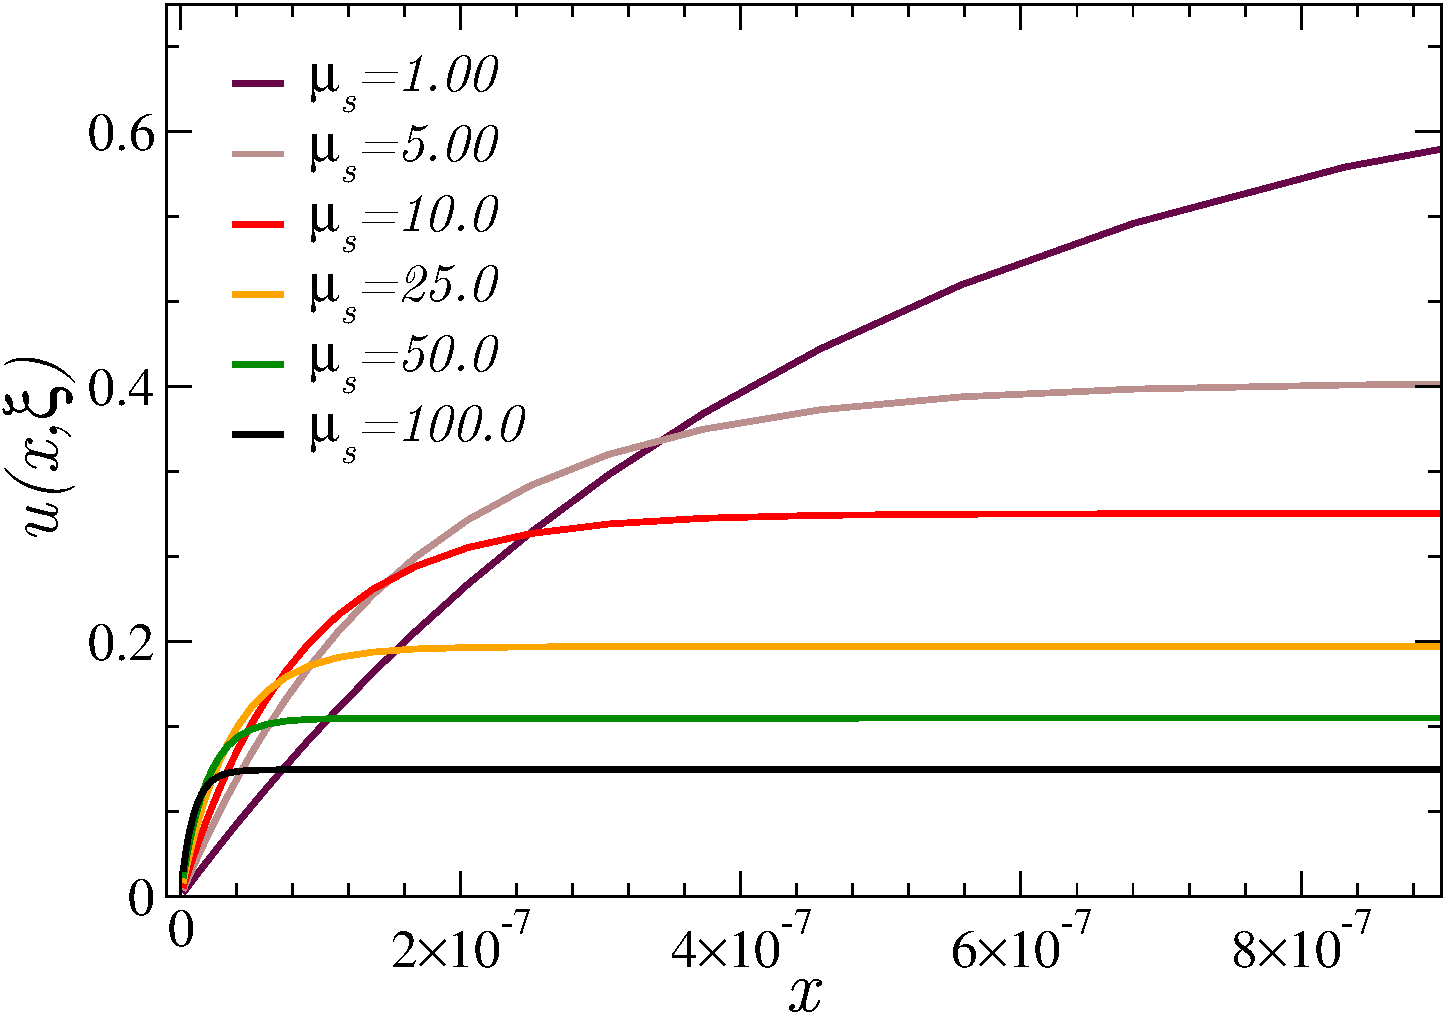
\includegraphics[width=1.0\textwidth]{figuras/blayers.pdf}\\
%\end{column}
%\begin{column}{0.5\textwidth}
%\centering
%  \includegraphics[width=1.0\textwidth]{figuras/xilay-eps-converted-to.pdf}\\
%\end{column}
%\end{columns}


\end{frame}

%%%%%%%%%%%%%%%%%%%%%%%%%%%%%%%%%%%%%%%%%%%%%%%%%%%%%%%%%%%%%%%%%%%%%%%%%

\begin{frame}
\frametitle{Capa límite}
%\begin{columns}[t]
%\begin{column}{0.33\textwidth}
%\centering
%  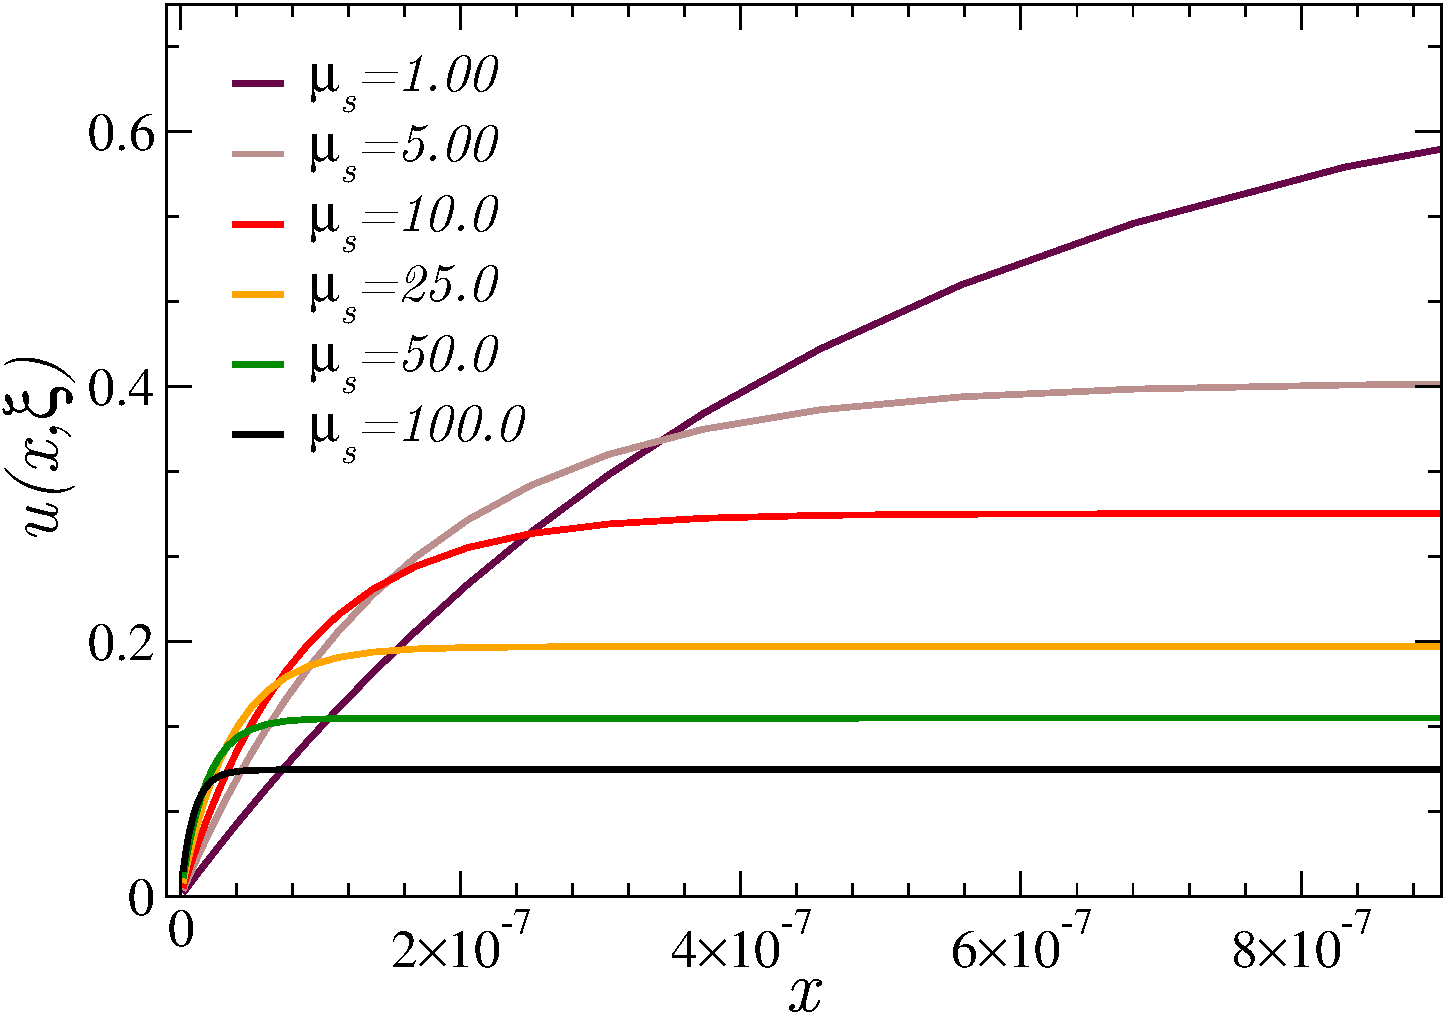
\includegraphics[width=1.1\textwidth]{figuras/blayers.pdf}\\
%   $\mu_a=q=1$
%\end{column}
%\begin{column}{0.5\textwidth}
\centering
  \includegraphics[width=1.0\textwidth]{figuras/xilay-eps-converted-to.pdf}\\
%\end{column}
%\begin{column}{0.5\textwidth}
%\centering
%  \includegraphics[width=1.0\textwidth]{figuras/xilay-eps-converted-to.pdf}\\
%\end{column}
%\end{columns}


\end{frame}

%%%%%%%%%%%%%%%%%%%%%%%%%%%%%%%%%%%%%%%%%%%%%%%%%%%%%%%%%%%%%%%%%%%%%%%%%

\begin{frame}
\frametitle{Capa límite}


       \begin{itemize}
           \item[$\bullet$] Gradientes
muy abruptos, que no pueden ser resueltos con los métodos estándar.

 
           \item[$\bullet$] Explicación física: valores pequeños de $\xi$ implican caminos geométricos largos.

           \item[$\bullet$] Identificamos las estructuras 
de capas límite.

           \item[$\bullet$] Las resolvimos mediante cambios de variables.

           \item[$\bullet$] Mediante el método propuesto 
           se logra resolver las capas límite con alto orden 
           y de forma muy eficiente: 400 puntos en contraste a 10000 puntos 
           requeridos por el esquema DD.
          
      \end{itemize}


\end{frame}
